\section{Higher-dimensional automata}
\label{sec:higher-dimensional-automata}

    %In the previous Section, we have enriched transition systems in order to take commutation of independent events into account. This commutation was formalized as an independence relation. Since this independence relation is a binary operator, it can only distinguish the mutual exclusion and non-interleaving concurrency of up to two events. What we would like is to generalize this notion of independence for an arbitrary number of events.
    
    %This
    The generalization of independence to $n$ events has lead to a geometric model for concurrency, studied by Pratt and van Glabbeek \cite{pratt91hda, Pratt00Sculptures, Glabbeek06HDA}. Pratt named this model Higher-Dimensional Automata (HDA) \cite{pratt91hda}. With higher-dimensional automata we can distinguish between the execution of $n$ non-interleaving concurrent events and of $n$ mutually exclusive events. Higher-dimensional automata are considered to be of high expressive power because of their property to distinguish $n$-events \cite{Kahl2013TheHG}. Hence, providing a generalization of differences, and common features, of various other models of concurrency, as done in \cite{Glabbeek06HDA} and \cite{Goubault18RelationshipsModelsForConcurrency}. Higher-dimensional automata also retain the state-based view and model the interleaving square with its interior filled, shown in Figure \ref{fig:HDA-filled-interleaving-square}. 
    
%    \ctlong{Do we want to consider Goubault's point in his PhD thesis about the unnatural way of extending the binary independence relation to n-ary. Requiring to solve the problem by going back to a geometric intuition.}
    
   A higher-dimensional automaton is a precubical set that encodes the independence of events by \emph{mappings}. Intuitively, we may consider a precubical set as $n$-dimensional cubes \cite{Fajstrup16DirectedAlgebraicTopologyConcurrency} together with their faces $-$ each $n$-dimensional cube has $2n$ faces. In other words, a front and a back face in each direction $i$ with $0 \leq i < n$. Mappings are families of functions that identify these faces, we call these \emph{face maps}. Face maps that satisfy the \emph{precubical identity} \cite{Fahrenberg05PhD, Fajstrup05DipathsInCubicalComplex, Fajstrup06AlgebraicTopologyConcurrency, Goubault2001TopologicalDeformHDA, goubault2003SomeGeometricPerspectives} are able to interpret the independence of events. In the concurrency theory literature, we find that the precubical identity is named the \emph{cubical law} \cite{Glabbeek06HDA, Johansen16STstruct}, since applications of algebraic topology are still being investigated in concurrency theory. Here, we will follow the topological notion, and use the naming precubical identity.

    Intuitively, the precubical identity is considered to be the idea of "\emph{filling in holes}" of a $n$-dimensional cube \cite[Section 2]{pratt91hda}. This notion is shown in Figure \ref{fig:HDA-filled-interleaving-square}, where the interior of the interleaving square is filled. With higher-dimensional automata we are able to capture the main characteristic of both transition systems and asynchronous transition systems by the notion of "\emph{filling in holes}".
    
%    \ctlong{I need to explain (a)cyclic and non-degenerate HDAs. May use definition from Christian's ST-structures paper}
    
  %  First, we will define precubical sets and the mappings of precubical sets. Later, we will provide the definition for HDAs in terms of precubical sets and their mappings. These models are expressive since they can encode commutations between any n-tuple of actions, as opposed to only pairs of actions. We will use similar notations and definitions as Fajstrup et al. \cite{Fajstrup16DirectedAlgebraicTopologyConcurrency} and Thomas Kahl \cite{Kahl2013TheHG}.
    
    %  For someone unfamiliar with these terms it might seem convoluted and abstract. However, by the end of this Section we hope to have made these terms clear by demonstrations and examples. We will use similar notations and definitions as Fajstrup et al. \cite{Fajstrup16DirectedAlgebraicTopologyConcurrency} and Thomas Kahl \cite{Kahl2013TheHG}.
  
    \begin{definition}[Precubical set]
        \label{def:precubical-set}
         A \emph{precubical set} is a graded set $\mathcal{X}= \bigcup_{ n\in \Nat} \mathcal{X}_n$, with $\mathcal{X}_n\cap \mathcal{X}_m= \emptyset$ for $n\ne m$, together with mappings $s_{ k, n}, t_{ k, n}:\mathcal{X}_n\to \mathcal{X}_{ n- 1}$, with $1\leq k\leq n$, satisfying the \emph{precubical identities}
         
         %$\delta_{ k, n}^\nu:\mathcal{X}_n\to \mathcal{X}_{ n- 1}$, $k = 1,\dots, n$, $\nu \in \{0, 1\}$, satisfying the \emph{precubical identity}
        
        \begin{equation*}
            \alpha_{ k, n- 1} \beta_{ \ell, n}= \beta_{ \ell- 1, n- 1} \alpha_{ k, n} \qquad(1 \leq k< \ell \leq n)
        \end{equation*}
        for $\alpha, \beta\in\{ s, t\}$.
    %    \begin{equation*}
    %        \delta_{ k, n- 1}^\nu \circ \delta_{ \ell, n}^\mu= \delta_{ \ell- 1, n- 1}^\mu \circ \delta_{ k, n}^\nu \qquad(\nu,\mu \in \{0,1\},\ k< \ell)\,.
    %    \end{equation*}
    \end{definition}
    
    A \emph{graded} set is a \emph{family of sets} where its elements are $n$-cells. A \emph{family of sets} is the disjoint union of these $n$-cells, $\mathcal{X}_n\cap \mathcal{X}_m= \emptyset$ for $n\ne m$. In the beginning of this Section, we called these $n$-cells for $n$-dimensional cubes. The naming $n$-dimensional cubes comes from Fajstrup et al. \cite{Fajstrup16DirectedAlgebraicTopologyConcurrency}, where $n$-dimensional cubes are precubical sets together with their faces. In this thesis, we will call elements of $\mathcal{X}_n$ for $n$-cells,  or simply cells, even though there are different names for these elements such as \emph{$n$-dimensional cubes} \cite{Pratt00Sculptures, Fajstrup16DirectedAlgebraicTopologyConcurrency}, \emph{$n$-transitions} \cite{Goubault95PhDThesis} and \emph{hypercubes} \cite{Glabbeek06HDA}. If $x \in \mathcal{X}_n$, then we say that $x$ is of dimension $n$ and is written $dim x = n$.
    
    The mappings $s_{ k, n}$ and $t_{ k, n}$  are called \emph{face maps}, and we will usually omit the extra subscript $n$ and simply write $s_k$ and $t_k$. Face maps are families of functions that identify the faces of the $n$-cells, in the same manner as described with $n$-dimensional cubes. Families of functions are usually considered as a set of functions whose equations have a similar form. However, in this context we will interpret them geometrically as faces of a cube.
    
    Each $n$-cell $x \in \mathcal{X}_n$ has \emph{$n$ lower faces $s_1 x,\dotsc, s_n x$} and \emph{$n$ upper faces $t_1 x,\dotsc, t_n x$}, and the precubical identity expresses the fact that ($n-1$)-faces of an $n$-cell meet in common ($n-2$)-faces, see Figure \ref{fig:precubical-set-interleaving-square-preidentity}.
    
    Figure \ref{fig:precubical-set-interleaving-square-geometric} and \ref{fig:precubical-set-interleaving-square-preidentity} represent a 2-cell showing both the four faces $s_1 x$, $t_1 x$, $s_2 x$, $t_2 x$ and the four possible mappings of the precubical identity. Figure \ref{fig:precubical-set-interleaving-square-geometric} is more of a geometrical picture of the 2-cell with its interior filled.
    
    \begin{figure}[ht]
        \centering
        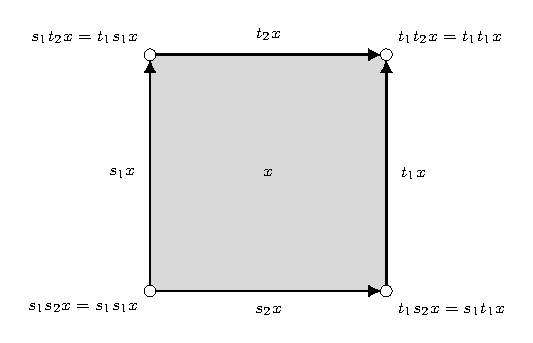
\includegraphics[scale=1.3]{Figures/3.An-introduction-to-non-interleaving-models-for-concurrency/precubical-square/cubical-law-2-cell-geometrical.pdf}
         \captionof{figure}[Geometric representation of a 2-cell]{We have a geometrical picturing of the 2-cell with its interior filled, four faces $s_1 x$, $t_1 x$, $s_2 x$, $t_2 x$ and four corners representing the mappings of the precubical identity.}
        \label{fig:precubical-set-interleaving-square-geometric}
    \end{figure}
    
    While, Figure \ref{fig:precubical-set-interleaving-square-preidentity} shows how the four mappings of the precubical identity is satisfied, and the fact that 1-faces of a 2-cell meet in common 0-faces.
    
    \begin{figure}[ht]
        \centering
        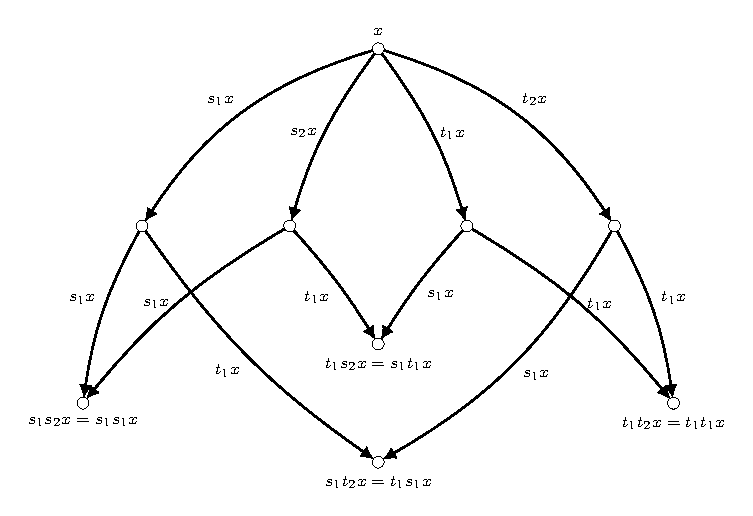
\includegraphics[scale=1]{Figures/3.An-introduction-to-non-interleaving-models-for-concurrency/precubical-square/cubical-law-2-cell-preidentity.pdf}
         \captionof{figure}[2-cell satisfying the precubical identities]{We have a 2-cell showing the four faces $s_1 x$, $t_1 x$, $s_2 x$, $t_2 x$ as edges and the four mappings of the precubical identity as the bottom nodes of the 2-cell.}
        \label{fig:precubical-set-interleaving-square-preidentity}
    \end{figure}
    
    We need a notion of \emph{morphisms} between precubical sets to be able to study the relationship between higher dimensional automata. From Section \ref{sec:ordinary-transition-systems}, we have that morphisms are considered to be simulations. Morphisms as simulation was an idea from Winskel and Nielsen in \cite{winskel95modelsCategory}. We want to extend morphisms to be structure-preserving maps that preserve orientation, shape, and time \cite[Section 2.2]{Goubault95PhDThesis}.
    
    Preserving orientation is addressed by \emph{directed} topology, where the object of study are topological spaces that have a sense of direction. Specifically, a topological space with a directed variant to incorporate the notion of irreversible time. Topology is a branch in mathematics that studies geometric shapes, and directed topology considered these geometric shapes to have a sense of direction. Shapes are preserved if we can present the geometry, we are interested in, as unions of \emph{points, segments, squares, cubes, ..., $n$-dimensional cubes} as collections of \emph{$n$-cells} ($n \in \mathbb{N}$). Preserving time means that we can reason about the directed variant and that every transition is mapped onto a transition.
    
    \begin{definition}[Morphism of precubical sets]
        \label{def:morphism-of-precubical-set}
        Morphisms $f: \mathcal{X}\to \mathcal{Y}$ of precubical sets are graded functions $f=\{ f_n: \mathcal{X}_n\to \mathcal{Y}_n\}_{ n\in \Nat}$ which commute with the face maps:
        
        \begin{equation*}
%            \alpha_k\circ f_n= f_{ n- 1}\circ \alpha_k for all n\in \Nat, k\in\{ 1,\dots, n\}, and \alpha\in\{ s, t\}.
            \alpha_k\circ f_n= f_{ n- 1}\circ \alpha_k \qquad\ \text{for all}\ n\in \Nat,\ k\in\{ 1,\dots, n\},\ \text{and}\ \alpha\in\{ s, t\}.
        \end{equation*}
    \end{definition}
    
    %A morphism $f: \mathcal{X} \to \mathcal{Y}$ is an \emph{embedding} if it is injective. In that case, we write $f: \mathcal{X} \hookrightarrow \mathcal{Y}$.

    Higher-dimensional automata are simply defined in terms of the precubical sets, and the relationship between higher-dimensional automata is described by the morphisms of the underlying precubical sets. Every figure presented thus far, may be considered as a higher-dimensional automata. We will from now on refer to the previous figures as higher-dimensional automata even though we first introduced them as transition systems, asynchronous transition systems and $n$-cells.
    
    %A \emph{higher-dimensional automaton} (HDA) is a precubical set $\mathcal{X}$ with a designated initial cell $i\in \mathcal{X}_0$.  Morphisms of higher-dimensional automata are precubical morphisms which fix the initial cell. For our definition of higher-dimensional automata, we will define it as presented by Van Glabbeek \cite{Glabbeek06HDA} and Johansen \cite{Johansen16STstruct}. However, the definition of higher-dimensional automata will interpret precubical sets and morphisms as defined earlier.
    
    % , a set of final cells, and a labelling function that attaches to each transition cell an action label respecting the condition that opposite faces of a square get the same label.
    
    %\ctlong{Precubical sets weren't defined as a tuple, what is the connection between HDA definition and precubical sets?}
    
    %\ctlong{Provide the set theoretic notion of HDA here and use van Glabbeek as reference}
    
    %\ctlong{Here write that Q corresponds to X, and s, t correspond to the value of $\mu$ and $\nu$ (0 or 1).}
    
    \begin{definition}[Higher-dimensional automata \cite{Glabbeek06HDA, Johansen16STstruct}]
        \label{def:higher-dimensional-automata}
        A precubical set $\mathcal{H} = (\mathcal{Q},s,t)$ is a precubical set $\mathcal{Q}$ together with $s$ and $t$ being the collection of all the face maps, that is, for all $n$. 
        
        A higher-dimensional automata is a tuple $(\mathcal{Q}, s, t, l, \mathcal{I}, \mathcal{F})$ over an alphabet $\Sigma$ such that $l(s_i(q)) = l(t_i(q))$ for all $q \in \mathcal{Q}_2$ and $i \in \{1,2\}$, and with a designated initial cell $\mathcal{I} \in \mathcal{Q}_0$ and $\mathcal{F} \subseteq \mathcal{Q}_0$ final cells.
%        A \emph{higher-dimensional automaton} (HDA) is a precubical set $\mathcal{Q}$ with a designated initial cell $q_0\in \mathcal{Q}_0$.
        
%        Morphisms of higher-dimensional automata are precubical morphisms which fix the initial cell. 
        
%        A morphism $f: \mathcal{X} \to \mathcal{Y}$ is an \emph{embedding} if it is injective. In that case, we write $f: \mathcal{X} \hookrightarrow \mathcal{Y}$.
    \end{definition}
    
    %In the following, we have that $\mathcal{Q}$ is a precubical set with $s$ and $t$ corresponding to $0$ and $1$, respectively. Similarly, to how we use $\nu, \mu \in \{0,1\}$ for the face maps for precubical sets. We fix the notion of start ($0$) and termination ($1$) of an execution to $s$ and $t$, respectively. $\mathcal{I}$ fixes the initial cell, like the precubical set with a designated initial cell $i \in \mathcal{X}_0$. $\mathcal{F}$ is the set of possible end states of the higher-dimensional automata that have to end in $\mathcal{Q}_0$. $l : \mathcal{Q} \rightarrow \mathcal{A}$ is the labelling function, where each one-dimensional transition, $\mathcal{Q}_1$, is labeled by an action from the alphabet $\mathcal{A}$.
    
    
    % We may consider a morphism as an \emph{embedding}, as follows:
    %\ctlong{What is the difference between embeddings and injective? Why defined here?!}

    %\begin{definition}[Morphisms as Embeddings]
    %    A morphism $f:\mathcal{X}\to \mathcal{Y}$ is an \emph{embedding} if it is injective; in that case we write $f: \mathcal{X} \hookrightarrow \mathcal{Y}$.
    %\end{definition}

    The concurrent execution of a higher-dimensional automata is modeled by including the two-dimensional surface. Intuitively, a concurrent execution can be seen as moving across the surface such that the execution preserves the directed variant, that is, to incorporate a notion of irreversible time. This is pictured in Figure \ref{fig:HDA-filled-interleaving-square}. 
    
    %The concurrent execution of a higher-dimensional automata is modeled by including the two-dimensional surface delineated by the one-dimensional $a$-transitions and $b$-transitions as a transition in the automata. This is pictured as
    
    \begin{figure}[ht]
        \centering
        \includegraphics[scale=1.2]{Figures/3.An-introduction-to-non-interleaving-models-for-concurrency/HDA_filled_interleaving_square/filled-interleaving-diamond.pdf}
         \captionof{figure}[Filled interleaving square]{Example of a HDA with four states, $q^1_0, q^2_0, q^3_0$ and $q^4_0$, four transitions, two of which are labeled $a$ and the other two are labeled $b$, and a surface, $q_2$. The surface represents the notion of "filling in holes" \cite[Section 2]{pratt91hda}, which is a continuous deformation of instructions $ab$ into $ba$, or vice versa.}
         %With this continuous deformation we can distinguish between mutually exclusive and non-interleaving concurrent events.}
        \label{fig:HDA-filled-interleaving-square}
    \end{figure}
    
    A computation is a path in this higher-dimensional automaton.
    
    \begin{definition}[Paths in HDAs \cite{Johansen16STstruct}]\label{def_paths_HDA}
        \label{def:paths-in-HDAs}
        A \emph{single step} in a HDA is either
        \begin{enumerate}
            \item $q_{n-1}\transition{s_{i}}q_{n}$ with $s_{i}(q_{n})=q_{n-1}$ or 
            \item $q_{n}\transition{t_{i}}q_{n-1}$ with $t_{i}(q_{n})=q_{n-1}$, 
        \end{enumerate}
        \noindent where $q_{n}\in \mathcal{Q}_{n}$ and $q_{n-1}\in \mathcal{Q}_{n-1}$ and $1\leq i\leq n$. 

        A \emph{path} $\pi\defequal q^{0}\transition{\alpha^{1}}q^{1}\transition{\alpha^{2}}q^{2}\transition{\alpha^{3}}\dots$ is a sequence of single steps $q^{j}\transition{\alpha^{j+1}}q^{j+1}$, with $\alpha^{j}\in\{s,t\}$. We say that $q\in\pi$ iff $q=q^{j}$ appears in one of the steps in $\pi$.  The first cell in a path is denoted $\startPath{\pi}$ and the ending cell in a finite path is $\finishPath{\pi}$. 
    \end{definition}
    
    The markings of the steps by $s$ may be seen as going from a lower cell to a higher cell, and steps by $t$ as the opposite, in the higher dimensional automaton. In many of the later proofs it is though useful to have the exact map easily visible, namely, the index that the step uses, rather than explicitly assuming the index every time. If there is no $\finishPath{\pi}$, then the path is infinite. When the index is not important we write $\transition{s}$ or $\transition{t}$.

    %Note that the marking of the steps by $s/t$ can be deduced from the fact that the step goes from a lower cell to a higher cell for $s$-steps, and the opposite for $t$-steps. It is though useful in many of the proofs to have easily visible the exact map, that is, the index that the step uses, instead of explicitly assuming it every time. If there is no $\finishPath{\pi}$, then the path is infinite. When the index is not important one writes $\transition{s}$ or $\transition{t}$.
    
    \begin{definition}[Histories for $\HDA$s \cite{Johansen16STstruct}]
    \label{def:histories-for-HDA}
    
        In a $\HDA$ two paths are \emph{adjacent}, denoted $\pi\adjacentHDA\pi'$, if one can be obtained from the other by replacing, for $q,q'\in \mathcal{Q}$ and $i<j$,
        
        \begin{enumerate}
            \item a segment $\transition{s_{i}}q\transition{s_{j}}$ by $\transition{s_{j-1}}q'\transition{s_{i}}$, or
            \item a segment $\transition{t_{j}}q\transition{t_{i}}$ by $\transition{t_{i}}q'\transition{t_{j-1}}$, or
            \item a segment $\transition{s_{i}}q\transition{t_{j}}$ by $\transition{t_{j-1}}q'\transition{s_{i}}$, or
            \item a segment $\transition{s_{j}}q\transition{t_{i}}$ by $\transition{t_{i}}q'\transition{s_{j-1}}$.
        \end{enumerate}

        Two finite paths are \textit{l-adjacent} $\pi\ladjacentHDA{l}\pi'$ when the segment replacement happens at position $l+1$; that is, $q$ is the $l+1$ cell in the path. \emph{Homotopy} is the reflexive and transitive closure of adjacency. Two homotopic paths are denoted $\pi\homotopicHDA\pi'$ and share their respective start and end cells. The homotopy class of a rooted path is denoted $\homotopyClass{\pi}$. A homotopy class with end cell $q$ is said to be \emph{a history of $q$}. One cell may have several histories, as is the case with the interleaving square $\HDA$ from Figure~\ref{fig:HDA-filled-interleaving-square}. Whenever a cell has a unique history we use the notation $\homotopyClass{q}$, instead of $\homotopyClass{\pi}$ with $\finishPath{\pi}=q$.
    \end{definition}

    Homotopy is defined for all paths such that a cell of higher dimension has a history in the same way that the inside of a square has a history. The homotopy is provided by Johansen in \cite{Johansen16STstruct}, where the homotopy is different compared to the definition in \cite[Section 1.6]{Goubault18RelationshipsModelsForConcurrency} because not only the state cells of dimension $0$, that is, vertices that form the corners of a cube, have histories, but also cells of higher dimensions.
    
    History unfoldings of process graphs have been defined by Van Glabbeek in \cite[Section 3]{Glabbeek96HistoryUnfolding}. Inspired by the definition of history unfoldings of process graphs, we will define the same notion for higher-dimensional automata. Johansen in \cite{Johansen16STstruct}, provides a definition of history unfolding for higher-dimensional automata which can be correlated with the definition of unfoldings from \cite{Glabbeek96HistoryUnfolding}. Also, alternative definitions of unfoldings for $\HDA$ can be found in \cite{Fahrenberg05PhD, Fahrenberg15PartialHDA}.

    \begin{definition}[History unfolding for HDAs]\label{def_unfolding_history} 
        The \emph{history unfolding} of a higher dimensional automaton $\mathcal{H}$ is a $\HDA$ denoted $\unfolding(\mathcal{H})$, respecting the cubical laws, as shown in \cite[Proposition 3.30]{Johansen16STstruct}, and given by:
        
        \begin{itemize}
            \item $Q_{n}^{\unfolding(\mathcal{H})}$ is the set of histories that end up in cells on level $Q_n$ of $\mathcal{H}$;
            \item has the labelling copied from $\mathcal{H}$: $l^{\unfolding(\mathcal{H})}(\homotopyClass{\pi})=l^{H}(\finishPath{\pi})$;
            \item initial cell the empty rooted history;
            \item the $s/t$ maps are built from the corresponding maps between the end cells of the histories: 
                \[
                    s_{i}(\homotopyClass{\pi})=\homotopyClass{\pi'}\mbox{\ \ \ iff\ \ \ }s_{i}(q)=q'\wedge \pi'\transition{s_{i}}\pi\wedge \finishPath{\pi'}=q'\wedge \finishPath{\pi}=q;
                \]
                \[
                    t_{i}(\homotopyClass{\pi})=\homotopyClass{\pi'} \mbox{\ \ \ iff\ \ \ } t_{i}(q)=q' \wedge \pi\transition{t_{i}}\pi' \wedge \finishPath{\pi'}=q'\wedge \finishPath{\pi}=q.
                \]
        \end{itemize}
    \end{definition}
    
    %In higher-dimensional automata there are often multiple histories that end up in the same cell, meaning that there are different ways of reaching the same cell. A history unfolding for higher-dimensional automata is then the histories that end up in the same cell, where the end of a history is the final cell. Intuitively, we may consider histories as paths that branch at the same cell and meet at the final cell.
    
    The notion of \emph{unfolding} removes iteration and is commonly used to turn a complicated model such as higher-dimensional automata into a simpler, but potentially infinite one. Unfolding is important in relation to the sculpting method introduced in Chapter \ref{chap:sculpting-in-concurrency}. For HDA this picture is more complicated.  Figure~\ref{fig:HDA-broken-box} (left) shows a simple HDA which is a sculpture. However, we will show that its unfolding (right) is \emph{not} a sculpture.

    \begin{definition}[Morphism of HDAs \cite{Johansen16STstruct}]
        \label{def:isomorphism-of-higher-dimensional-automata}
        A morphism between two \emph{HDA}s, $f : \mathcal{H} \rightarrow \mathcal{H}'$ is a dimension preserving map between their cells $f : \mathcal{Q} \rightarrow \mathcal{Q}'$, such that:
        
        \begin{enumerate}
            \item the initial cell is preserved: $f(\mathcal{I}) = \mathcal{I}'$
            \item the labelling is preserved: $l'(f(q_1)) = l(q_1)$ for all $q_1 \in \mathcal{Q}_1$,
            \item the mappings are preserved, for any $q_n \in \mathcal{Q}_n$ and $1 \leq i \leq n$:
            \begin{itemize}
                \item $s'_i(f(q_n)) = f(s_i(q_n))$ and
                \item $t'_i(f(q_n)) = f(t_i(q_n))$.
            \end{itemize}
        \end{enumerate}
        
        When a morphism is bijective we call it isomorphism. Two HDAs are isomorphic, denoted $\mathcal{H} \cong \mathcal{H}'$, when there exists an isomorphism between them.
    \end{definition}

    We write $\allHDA$ for the category of higher-dimensional automata, where the object of the category are higher-dimensional automata and morphisms are as defined in Definition \ref{def:isomorphism-of-higher-dimensional-automata}.
    
    In the definition of precubical sets, we consider them to be non-degenerate. Many of the results from this thesis assumes higher-dimensional automata to be non-degenerate. Also, we consider the directed variant, mentioned so far, to be higher-dimensional automata that are acyclic. Johansen in \cite{Johansen16STstruct}, defines these notions for higher dimensional automata:
    
    \begin{definition}[Acyclic and non-degnerate HDAs \cite{Johansen16STstruct}]
        \label{def:acyclic-and-non-degenerate-higher-dimensional-automata}
        A higher-dimensional automata is called acyclic if no path visits a cell twice. A higher-dimensional automata is non-degenerate if for any cell $q$ all its faces exist and are different, in the sense of $\forall i \neq j : \alpha_i(q) \neq \beta_i(q) \wedge \alpha , \beta \{s,t\}$, no two transitions with the same label share both their end states.
    \end{definition}
    
    The notion of acyclic does not allow cycles, or loops, in the higher-dimensional automata, and the notion of non-degeneracies is related to the underlying precubical sets\footnote{In topology, The distinction between non-degeneracies and degeneracies are subtle and will not be considered here. In \cite{Goubault95PhDThesis}, the  distinction between non-degeneracies and degeneracies is considered.}. The restriction on higher-dimensional automata being non-degenerate is similar to that of Fajstrup et al. \cite{Fajstrup16DirectedAlgebraicTopologyConcurrency} and that of van Glabbeek \cite{Glabbeek06HDA}. Also, the restriction above is the same for precubical sets where two opposite s-maps and t-maps can be equal, such that $s_i(q) = t_i(q)$ is allowed. We assume all s-maps and t-maps are to be total, as done in \cite{Johansen16STstruct}. A study of partial higher-dimensional automata, where s-maps and t-maps are partial, has been considered by Fahrenberg in \cite{Fahrenberg15PartialHDA}.
    
    %When higher-dimensional automata are required to be acyclic, then the non-degeneracy restriction is ruled out since it would create a cycle.
    
    %Because of these restrictions of higher-dimensional being acyclic and non-degenerate, we silently assume all s-maps and t-amps to be total. A study of partial higher-dimensional automata, where s-maps and t-maps are partial, has been considered by Fahrenberg in \cite{Fahrenberg15PartialHDA}.
    
    
  %  \ctlong{Do we need to define HDA histories and unfoldings here?!}

    %\ctlong{Add the figure 1 from sculpting paper by Uli and Christian}
    
%    HDAs are considered to be of high expressive power because of their property to distinguish $n$-events, thus providing a general framework for studying difference and common features of various other models of concurrency. However, capturing the exact class of HDAs, in which events can be identified precisely, using the standard method used in the literature, that is, as transitions opposite \cite{?}, seems to be challenging. We know from the work by Johansen in \cite{Johansen16STstruct} on ST-structures, the event-based counterpart of HDAs, that HDAs are generally not good at identifying events. Also from his work, the ST-structures are well suited to represent the events, thus overcoming the problem identified in \cite[Figure 5]{Johansen16STstruct} (e.g., the Asymmetric Conflict) where events cannot be represented as a HDA, but faithfully represented as an ST-structure. Going further, ST-structures are one response to the event-state duality of Pratt \cite{Pratt00Sculptures} in HDA. \ctlong{Need to reword this!}
    
   % ST-structures, which is the event-based counterpart of higher-dimensional automata, we able to identify the precedence of events. ST-structures extend configuration structures with the notion of "during" as opposed to only talking about "what happens after" an event. Therefore, in ST-structures we can see when an event, or several concurrent ones, are currently being executed, as well as when the event has terminated its execution. In \cite{Johansen16STstruct}, it suggests that a main characteristic of higher-dimensional automata is captured by ST-structures, opposed to the standard configuration structures; this is the power to look at the currently executing concurrent events (not only observe their termination).
    
%    Identify the precise class of HDAs which events can be indentified precisely using the standard method used in the literature, that is, as transitions opposite in a square \cite{?}. From the work in \cite{Johansen16STstruct} on ST-structures, which are the event-based counterpart of HDAs, we know that HDAs are generally not good at identifying events. However, as shown in this paper, the sculptures are well suited to represents the events too, thus overcoming the problem identified in \cite[Figure 5]{Johansen16STstruct} (e.g., the Asymmetric Conflict) cannot be represented as HDA but can be faithfully represented as a sculpture and as a ST-structure. Going further, sculptures are one response to the event-state duality of  Pratt \cite{Pratt02eventStateDuality} in HDA. One sees the HDA as a state-based model, similar to classical automata and labelled transition systems, whereas the ST-structure are an event-based model, similar to event structures, which was developed to be the event-based counterpart of HDAs. In this line of research, sculptures manage to identify exactly the vents that are intrinsically captured by HDAs, and correspond exactly to the ST-structures (see Section~\ref{?}).
    
    

    
%    Interestingly, the resulting models are \emph{algebraic structures} which can be interpreted roughly as \emph{topological spaces}. However, as pointed out by Fahrenberg in \cite{Fahrenberg05PhD}, there is a problem with the translation from higher-dimensional automata to topological spaces: one looses all information concerning precedence of events. In order to make this connection precise, it turns out that topological spaces are not exactly the right notion for our purpose. One needs to use a \emph{directed variant}, that is, to incorporate a notion of irreversible time. This and other problems are addressed in directed topology, where the objects of study are topological spaces equipped with precedence information \cite{Fahrenberg05PhD, Goubault95PhDThesis, Fajstrup16DirectedAlgebraicTopologyConcurrency} (cf. \cite{?}).
    
  %  However, with ST-structures, which is the event-based counterpart of higher-dimensional automata, we able to identify the precedence of events. ST-structures extend configuration structures with the notion of "during" as opposed to only talking about "what happens after" an event. Therefore, in ST-structures we can see when an event, or several concurrent ones, are currently being executed, as well as when the event has terminated its execution. In \cite{Johansen16STstruct}, it suggests that a main characteristic of higher-dimensional automata is captured by ST-structures, opposed to the standard configuration structures; this is the power to look at the currently executing concurrent events (not only observe their termination).


%    Interestingly, the resulting models are \emph{algebraic structures} which can be interpreted geometrically roughly as \emph{topological spaces} in which paths correspond to executions and two executions are equivalent when the corresponding paths are \emph{homotopic}, that is, connected by a continuous deformation from one to the other. There is however a problem with the translation from higher-dimensional automata to topological spaces: one looses all information concerning precedence of events. In order to make this connection precise, it turns out that topological spaces are note exactly the right notion for our purpose. One needs to use a \emph{directed variant}, that is, to incorporate a notion of irreverssible time. This and other problems is addressed in directed topology, where the objects of study are topological spaces equipped with precedence information.
    
 %   However, with event-based models such as configuration structures \cite{NielsenPW79eventstructures, GlabbeekP09configStruct}, event structures \cite{NielsenPW79eventstructures, Winskel86} and unrestricted event structures \cite{GlabbeekP95config, GlabbeekP09configStruct}, 
    
  %  In order to make this connection precise, it turns out that topological spaces are not exactly the right notion for our purpose. One needs to use a \emph{directed variant}, that is, to incorporate a notion of irreversible time.
        
 %  \ctlong{Notes taken from Uli's PHD thesis:}
   % A higher-dimensional automaton is basically a precubical set, and as such it has a \emph{geometric realization} as a topological space.
    
  %  There is however a problem with translation from higher-dimensional automata to topological spaces: one loses all information concerning precedence of events. In a higher-dimensional automaton, there are causal relationships between states or transitions, but a topological space is symmetric, so these non-symmetric relations are lost in the translation.
    
  % This and other problems are addressed in directed topology, where the objects of study are topological spaces equipped with precedence information.
    
  %  \begin{itemize}
  %     \item Po-spaces and local po-spaces by Lisbeth Fajstrup, Eric Goubault
  %      \item d-spaces by Marco Grandis
   %     \item Flow by Philippe Gaucher
  %      \item Streams by Sanjecvi
  %  \end{itemize}
    
  %  One is often interested in relations between concurrent systems, especially in equivalences of concurrent systems. These come in two flavours: observational and behavioral, and form a topological viewpoint, the latter is more interesting.

  %  \ctlong{Need to continue on the path of figuring out why these HDAs are not good at identifying events. Need to present this at the end of this Section as a build up to the next Section on ST-structures. I want to present ST-structures as an attempt to identify events in HDAs.}
    
  %  We see the notion of configuration (in its various guises \cite{NielsenPW79eventstructures, GlabbeekP09configStruct}) as fundamental to event-based models. The configuration structures, introduced in \cite{GlabbeekP95config}, are a rather general model of concurrency based on sets of events (forming the configurations of the modelled system). A thorough study of the generality and expressiveness of configuration structure is carried out in \cite{GlabbeekP09configStruct} where relations with general forms of event structures are made (where the pure event structures are the more well behaved, instances of which are found in the literature). The configuration structures lend themselves easily to action refinement, as studied in \cite{GlabbeekG01refinement}, which makes them an ideal candidate for incremental development of concurrent systems where the system architecture start with an abstract model which is subsequently refined to more concrete instances.
    
 %   We think that a main characteristic of higher-dimensional automata is captured by ST-structures, opposed to the standard configuration structure; this is the power to look at the currently executing concurrent events (not only observe their termination). In other words, we can now talk about what happens 'during' the concurrent execution of one or more events.
    
 %   ST-structures extend configuration structures with the notion of "during" as opposed to only talking about "what happens after" an event. Therefore, with ST-structures we can see when an event, or several concurrent ones, are currently being executed, as well as when the event has terminated its execution. More technically, configuration structures are those ST-structures where "during" is irrelevant, that is, where events are always terminated.
    
 %   When computational steps are also considered, together with the property of connectedness, then configuration structures impose that concurrency square are always "filled in". This suggests that configuration structures are not adequate for distinguishing between the interleaving an concurrency of two events (not labels), because the interleaving square cannot be empty.
    
  %  In response, we see when comparing ST-structures with the unrestricted event structures of \cite{GlabbeekP09configStruct} that the latter can capture the empty interleaving squares, and thus do right justice to distinction that Pratt advocates for between notion of concurrency and interleaving, at the level of events even, not only at the level of the labels.
    
  %  Still, for unrestricted event structures we see that the concurrency steps will always be fully filled in. This is made obvious by the property of ST-structures called "adjacent-closure" (which, as the name suggests, is closed relation to the similar notion of adjacency for HDAs).
    
 %  In the event-based models, configurations are capturing the state of the system. For configuration structures these correspond to only the corners of a HDA, that is, cells of dimension 0, where the ST-configurations correspond to any higher-dimensional cell in a HDA. Therefore, we may expect that when looking at acyclic HDAs to find the ST-structures.
    
  %  In particular, the property of adjacent-closure of ST-structures corresponding to HDAs being non-degenerate (i.e., having for a cell/cube all the faces nicely in place).
    
  %  But it turns out that neither of these can be embedded in the other. For HDAs it is easy to see because ST-structures only capture unfoldings. For the opposite, it turns out that the classical way of identifying events in HDAs (as parallel boundaries of a square) is not enough to express the way ST-structures can work with events.
    
 %   It is known that configuration structures correspond to Chu spaces over 2. The extension of "duration" that ST-structures represent in turn corresponds to the extension of Chu spaces to being defined over 3, since the structure 3 is the extension of 2, which is the simple "start < terminate", to the "start < during < terminate".
    
  %  It could be interesting to look at Chu spaces as isomorphic to ST-structures through the result of this Section.
    
%    \begin{definition}[cubical set]
 %       A \emph{cubical set} consists of a family of sets ($Q_{n})_{n \leq 0}$ and for every $n \in \mathbb{N}$ a family of maps $s_{i}, t_{i} : Q_{n} \rightarrow Q_{n-1}$ for $1 \leq i \leq n$, such that
 %       \begin{center}
 %           $\alpha_{i} \circ \beta_{j} = \beta_{j-1} \circ \alpha_{i}$ \indent for all $1 \leq i < j \leq n$ and $\alpha, \beta \in \{s,t\}$.
 %       \end{center}
 %   \end{definition}
    
 %   \ctlong{Ask Christian if I should use the definition from Van Glabbeek or the one from Directed Algebraic Topology and Concurrency book?}

    % Higher-dimensional automata are considered an extension of both transition systems and asynchronous transition systems. With higher-dimensional automata we can distinguish between the execution of $n$ non-interleaving concurrent actions and of $n$ mutually exclusive actions.
    
    %From the paper by Pratt, where he advocates for modeling concurrency with geometry arises a model named higher-dimensional automata. This is from the thesis of wanting to have both branching time and non-interleaving concurrency described together in a single geometric model. We considered the transition system as a one-dimensional space consisting of edges (its transitions) meeting and branching at vertices (its states). Non-interleaving concurrency is represented by dimension: an n-dimensional cell (element of space) is used to represent the concurrent execution of n sequential processes, and its boundaries represent the starting or halting of some of those processes.
    
    %HDAs were defined first as n-complexes and in a categorical way, but has later developed to be n-cells, cubical complex or precubical sets.
    
    %Our original defnition of HDA was based on n-categories. These are discrete higher-dimensional structures where n-cells have only two boundaries, source and target (domain and co-domain), independent of n.
    
   % Discussions with Rob van Glabbeek shortly after the appearance of (Pratt91) convinced me that n-cubes were preferable to either n-globs or n-simplices as the basic n-cells representing the concurrent execution of n events, and also led to his note (van Glabbeek - bisimulation for HDA 1991).
    
    %\begin{definition}[cubical set]
   %     A \emph{cubical set} consists of a family of sets ($Q_{n})_{n \leq 0}$ and for every $n \in \mathbb{N}$ a family of maps $s_{i}, t_{i} : Q_{n} \rightarrow Q_{n-1}$ for $1 \leq i \leq n$, such that
  %      \begin{center}
   %         $\alpha_{i} \circ \beta_{j} = \beta_{j-1} \circ \alpha_{i}$ \indent for all $1 \leq i < j \leq n$ and $\alpha, \beta \in \{s,t\}$.
    %    \end{center}
   % \end{definition}
    
   % \cjlong{Definition from Van Glabbeek. This will be our first definition with cubical sets as basis, but later we will provide the new definition of HDA with precubical sets as basis. This has to do with cubical sets also have some embedding maps, corresponding to the projection maps that precubical sets have. Uli has the exact definition in his papers, because in topology they are very careful with this distinction, whereas in computer science (and my older papers) they ignored this difference.}

    %\begin{definition}[higher-dimensional automata]
    %    An HDA, labelled over an alphabet A, is a tuple (Q,s,t,I,F,l) with (Q,s,t) a precubical set, $I \in Q_{0}, F \subseteq Q_{0}$ and $l:Q_{1} \rightarrow A$, such that $l(s_{i}(q)) = l(t_{i}(q))$ for all $q \in Q_{2}$ and $i = 1,2$.
    %\end{definition}
    
    % PHD of Eric Goubault
    %Geometry has been suggested as a tool for modeling concurrency using higher-dimensional objects to describe the concurrent execution of processes. This contrasts with earlier models based on interleaving of computation steps to capture all possible behaviours of a concurrent system. Such models must necessarily commit themselves to a specific choice of \emph{atomic action} which makes them unable to distinguish between the execution of two truly concurrent actions and of two mutually exclusive actions as there are both modeled by their interleaving. This contrasts also with models of true concurrency for which the asynchronous executions are not "first-class" transitions. This was the case of asynchronous transition systems (see Chapter 1) for which we have an independence relation but no notion of "real" asynchronous execution.
    
    % Pratt HDA Revisited.
    %The geometrical view of automata is implicit in A. Mazurkiewicz's algebraic notation of independence via partial monoids \cite{mazurkiewiz77traces, Mazurkiewicz84traces}. It is made more explicit and put to practical use in C. Papadimitriou's model for database concurrency control \cite{Papadimitriou86database}, with however no accompanying formal notion of an automaton. Higher-dimensional transitions make a brief apperance at the end of M. Shields' paper on deterministic asynchronous automata \cite{Shields85}. The explicit notion of higher-dimensional automaton as an extension of traditional automata theory was introduced by Vaughan Pratt at POPL'91 \cite{pratt91hda}. HDAs are an extension of asynchronous semantics.

   % In \cite{pratt91hda} and \cite{Glabbeek06HDA} Pratt and van Glabbeek advocate a model of concurrency based on geometry and in particular on the notion of a higher-dimensional automata (HDA). Higher-dimensional automata are generalizations of the usual non-deterministic finite automata as described in e.g. \cite{HopcroftUllman79AutomataTheory}. The basic idea is to use the higher dimensions to represent the concurrent execution of processes. Thus for two processes, $e_{1}$ and $e_{2}$, we model the mutual exclusive execution of $e_{1}$ and $e_{2}$ by the automaton
    
    %whereas their concurrent execution is modeled by including the two-dimensional surface delineated by the (one-dimensional)$e_{1}$- and $e_{2}$-transitions as a transition in the automaton. This is pictured as
    
    %\begin{figure}[H]
    %    \centering
    %    \includegraphics[scale=1.5]{master_thesis/Figures/1.Introduction/filled_interleaving_square/filled-interleaving-diamond.pdf}
    %    \caption{Filled interleaving square}
    %    \label{fig:HDA-filled-Interleaving-square}
    %\end{figure}
    
    %A computation is a path in this higher-dimensional automaton.

% Pratt HDA Revisited.
%The geometrical view of automata is implicit in A. Mazurkiewicz's algebraic notation of independence via partial monoids \cite{mazurkiewiz77traces, Mazurkiewicz84traces}. It is made more explicit and put to practical use in C. Papadimitriou's model for database concurrency control \cite{Papadimitriou86database}, with however no accompanying formal notion of an automaton. Higher-dimensional transitions make a brief apperance at the end of M. Shields' paper on deterministic asynchronous automata \cite{Shields85}. The explicit notion of higher-dimensional automaton as an extension of traditional automata theory was introduced by Vaughan Pratt at POPL'91 \cite{pratt91hda}. HDAs are an extension of asynchronous semantics.

%We arrived at the idea of "filling in the holes" of traditional automata by noticing a paradox implicit in the main theorem of \cite{NielsenPW81eventstructures}, the duality of prime event structures as event schedules and prime algebraic domains as state automata dual to schedules. While the event structures of the paper interpreted as schedules, were by design a model of true concurrency, their dual prime algebraic domains were unmistakably automata of the "false concurrency" kind, with Figure 1 a case in point having \{00, 01, 10, 11\} as its family of configurations. A perfect duality between true an false models of concurrency is paradoxical: for this distinction to be meaningful there must be something missing from the interpretation of prime algebraic domains as conventional automata.

%One evident difference between schedules and automata is that with the former the passage from $a \leq b$ to $b \leq a$ can be accomplished by moving a and b smoothly past each other in time. We asked what was the dual of this smoothness for automata. Somehow the $ab$ path must transform smoothly into the $ba$ path. The only sensible way this could happen was via a surface connecting the two. Familiarity with the geometric representation of natural tranformations of two functors, namely as 2-cells between those two functors viewed as two 1-cells having a common start and end, facilitated our arrival at this picture.
%%%%%

%\ctlong{Begining of new part from Sculpting paper.}
% On sculpting, Uli, Christian and me